% Template for Elsevier CRC journal article
% version 1.1-5p dated 18 January 2011
% SEM ACENTUACAO PROBLEMA UTF-8 : NAO ACEITA

% This file (c) 2010-2011 Elsevier Ltd.  Modifications may be freely made,
% provided the edited file is saved under a different name

% This file contains modifications for Procedia Computer Science
% but may easily be adapted to other journals

% Changes since version 1.0
% - elsarticle class option changed from 1p to 3p (to better reflect CRC layout)
% - this version uses option 5p for larger-format journals (text area 24.1 x 18.4 cm)

%-----------------------------------------------------------------------------------

%% This template uses the elsarticle.cls document class and the extension package ecrc.sty
%% For full documentation on usage of elsarticle.cls, consult the documentation "elsdoc.pdf"
%% Further resources available at http://www.elsevier.com/latex

%-----------------------------------------------------------------------------------

%%%%%%%%%%%%%%%%%%%%%%%%%%%%%%%%%%%%%%%%%%%%%%
%%%%%%%%%%%%%%%%%%%%%%%%%%%%%%%%%%%%%%%%%%%%%%
%%                                          %%
%% Important note on usage                  %%
%% -----------------------                  %%
%% This file must be compiled with PDFLaTeX %%
%% Using standard LaTeX will not work!      %%
%%                                          %%
%%%%%%%%%%%%%%%%%%%%%%%%%%%%%%%%%%%%%%%%%%%%%%
%%%%%%%%%%%%%%%%%%%%%%%%%%%%%%%%%%%%%%%%%%%%%%

%% The '5p' and 'times' class options of elsarticle are used for Elsevier CRC
\documentclass[5p,times,authoryear]{elsarticle}

%% The `ecrc' package must be called to make the CRC functionality available
%% ecrc_RIAI es el paquete ecrc de Elsevier con modificaciones para la revista RIAI
\usepackage{ecrc_RIAI}

%% The ecrc package defines commands needed for running heads and logos.
%% For running heads, you can set the journal name, the volume, the starting page and the authors

%%%%%%%%%%%%%%%%%%%%%%%%%%%%%%%%% Aaadido por Secretaraa RIAI
\usepackage[spanish]{babel}     % Idioma
\addto\captionsspanish{%
\def\tablename{Tabla}%
}
\usepackage[latin1]{inputenc}   % Lengua latina
\usepackage{amsmath}            % Para las referencias a ecuaciones con \eqref
\usepackage{epstopdf}           % Para poder insertar figuras .eps al compilar con PDFLATEX
\usepackage{flushend}           % Para igualar las columnas de la altima pagina
%\usepackage{hyperref}           % Para hipervanculos dentro del PDF
%%%%%%%%%%%%%%%%%%%%%%%%%%%%%%%%%%%%%%%%%%%%%%%%%%%%%%%


%% set the volume if you know. Otherwise `00'
\volume{00}

%% set the starting page if not 1
\firstpage{1}

%% Give the name of the journal
\journalname{Revista Iberoamericana de Automatica e Informática industrial}

%% Give the author list to appear in the running head
%% Example \runauth{C.V. Radhakrishnan et al.}
\runauth{Primer autor et al.}

%% The choice of journal logo is determined by the \jid and \jnltitlelogo commands.
%% A user-supplied logo with the name <\jid>logo.pdf will be inserted if present.
%% e.g. if \jid{yspmi} the system will look for a file yspmilogo.pdf
%% Otherwise the content of \jnltitlelogo will be set between horizontal lines as a default logo

%% Give the abbreviation of the Journal. Contast the Publisher if in doubt what this is.
\jid{RIAI}

%% Give a short journal name for the dummy logo (if needed)
\jnltitlelogo{}

%% Hereafter the template follows `elsarticle'.
%% For more details see the existing template files elsarticle-template-harv.tex and elsarticle-template-num.tex.

%% Elsevier CRC generally uses a numbered reference style
%% For this, the conventions of elsarticle-template-num.tex should be followed (included below)
%% If using BibTeX, use the style file elsarticle-num.bst

%% End of ecrc-specific commands
%%%%%%%%%%%%%%%%%%%%%%%%%%%%%%%%%%%%%%%%%%%%%%%%%%%%%%%%%%%%%%%%%%%%%%%%%%

%% The amssymb package provides various useful mathematical symbols
\usepackage{amssymb}
%% The amsthm package provides extended theorem environments
%% \usepackage{amsthm}

%% The lineno packages adds line numbers. Start line numbering with
%% \begin{linenumbers}, end it with \end{linenumbers}. Or switch it on
%% for the whole article with \linenumbers after \end{frontmatter}.
%% \usepackage{lineno}

%% natbib.sty is loaded by default. However, natbib options can be
%% provided with \biboptions{...} command. Following options are
%% valid:

%%   round  -  round parentheses are used (default)
%%   square -  square brackets are used   [option]
%%   curly  -  curly braces are used      {option}
%%   angle  -  angle brackets are used    <option>
%%   semicolon  -  multiple citations separated by semi-colon
%%   colon  - same as semicolon, an earlier confusion
%%   comma  -  separated by comma
%%   numbers-  selects numerical citations
%%   super  -  numerical citations as superscripts
%%   sort   -  sorts multiple citations according to order in ref. list
%%   sort&compress   -  like sort, but also compresses numerical citations
%%   compress - compresses without sorting
%%
%% \biboptions{comma,round}

% \biboptions{}

% if you have landscape tables
\usepackage[figuresright]{rotating}

% put your own definitions here:
%   \newcommand{\cZ}{\cal{Z}}
%   \newtheorem{def}{Definition}[section]
%   ...

% add words to TeX's hyphenation exception list
%\hyphenation{author another created financial paper re-commend-ed Post-Script}

% para poder introducir varias figuras que ocupen el ancho de las dos columnas.
\usepackage{subfigure}

% declarations for front matter

\begin{document}

\begin{frontmatter}

%% Title, authors and addresses

%% use the tnoteref command within \title for footnotes;
%% use the tnotetext command for the associated footnote;

%% use the fnref command within \author or \address for footnotes;
%% use the fntext command for the associated footnote;

%% use the corref command within \author for corresponding author footnotes;
%% use the cortext command for the associated footnote;
%% use the ead command for the email address,
%% and the form \ead[url] for the home page:
%%
%% \title{Title\tnoteref{label1}}
%% \tnotetext[label1]{}
%% \author{Name\corref{cor1}\fnref{label2}}
%% \ead{email address}
%% \ead[url]{home page}
%% \fntext[label2]{}
%% \cortext[cor1]{}
%% \address{Address\fnref{label3}}
%% \fntext[label3]{}

%\dochead{Cabecera artaculo}
%% Use \dochead if there is an article header, e.g. \dochead{Short communication}

\title{Preparacian de Artaculos para la revista RIAI:\\
Use Tipo Tatulo para el Tatulo del Artaculo}


%% use optional labels to link authors explicitly to addresses:
%% \author[label1,label2]{<author name>}
%% \address[label1]{<address>}
%% \address[label2]{<address>}

\author[First]{Primer A. Autor\corref{cor1}\fnref{label2}}
\ead{autor@cea-ifac.es}
\ead[url]{www.cea-ifac.es}

\author[Second]{Segundo B. Autor, Jr.}
\ead{autor2@cea-ifac.es}
\ead[url]{www2.cea-ifac.es}

\author[Third]{Tercer C. Autor}
\ead{autor3@cea-ifac.es}

\fntext[label2]{Nota al pie para el autor 1}
\cortext[cor1]{Autor en correspondencia.}


\address[First]{Comita Espaaol de Automatica, Parc Tecnologic de Barcelona, Edifici U, C/ Llorens i Artigas, 4-6, 08028 Barcelona, Espaaa. }
\address[Second]{Departamento de Automatica, Ingenieraa Electranica e Informatica, Universidad Politacnica de Madrid,  C/ Josa Gutiarrez Abascal, na2, 28006, Madrid,  Espaaa.}
\address[Third]{Departamento de Ingenieraa de Sistemas y Automatica,  Universitat Politacnica de Valencia, Camino de Vera, na14, 46022, Valencia, Espaaa.}

\begin{abstract}
%% Text of abstract
Estas instrucciones constituyen una guaa para la preparacian de
artaculos para la revista RIAI. Utilice este documento como un
conjunto de instrucciones. Tambian puede usarse como
una ``plantilla'' para preparar su manuscrito. Para las directrices
de envao, siga las instrucciones del sistema de envao de artaculos
de la pagina web de la revista. \emph{Copyright {\copyright} XXXX CEA. Publicado por Elsevier Espaaa, S.L. Todos los derechos reservados.}
\end{abstract}

\begin{keyword}
%% keywords here, in the form: keyword \sep keyword

%% MSC codes here, in the form: \MSC code \sep code
%% or \MSC[2008] code \sep code (2000 is the default)

palabra 1 \sep palabra 2 \sep 5-10 palabras clave (tomadas de la lista del sitio web de IFAC).

\end{keyword}

\end{frontmatter}

%%
%% Start line numbering here if you want
%%
% \linenumbers

%% main text
\section{Introduccian}
Estas instrucciones constituyen una guaa para la preparacian de
artaculos para la revista RIAI. Utilice este documento como un
conjunto de instrucciones. Puede usar este documento como
una ``plantilla'' para preparar su manuscrito en Latex. Para las directrices
de envao, siga las instrucciones del sistema de envao de artaculos
de la pagina web de la revista.
 {\bf{\emph {No cambie el tamaao de las fuentes o espaciado de lanea para introducir mas texto en un namero limitado de paginas}}}.  Utilice cursiva para enfatizar; no subraye.

\subsection{Una subseccian de ejemplo.}
Bifurcacian: Trazado del maximo local de $x$ con una disminucian de amortiguamiento $a$ (Fig.~\ref{fig1}).

Para insertar imagenes en \emph{Word}, posicione el cursor en el punto de insercian y o bien utilice Insertar | Imagen | Desde Fichero o copie la imagen al portapapeles de Windows y entonces use Editar | Pegado especial | Imagen (con ``Flotar sobre el texto'' deseleccionado).

RIAI no realizara ninguna operacian de formateado final a su artaculo. Su documento debe estar ``listo para filmar''. El namero lamite de hojas para el documento es de doce. {\bf Por favor, no modifique los margenes. Si esta creando el documento usted mismo, tenga en cuenta los margenes listados en la Tabla 1.}

\section{Procedimiento para el Envao de Artaculos}

Recuerde que RIAI esta considerado como un \emph{Camera Ready Copy Journal (CRC)}. Esto implica que los autores son responsables de aplicar el formato correspondiente a sus contribuciones. Desde la secretaraa de la revista no se ejecutara ninguna accian de formateo a los artaculos. A continuacian vemos unas subsecciones.

\subsection{Fase de Revisian}

Por favor, use este documento como una ``plantilla'' para preparar su documento. Para las directrices de envao, siga las instrucciones del sistema de envao de artaculos.

Dado que el lamite de paginas es de doce, es mejor preparar el envao inicial en el formato listo para filmar, de tal manera que tenga una buena estimacian de la longitud de hojas. Adicionalmente, el esfuerzo requerido para el envao de la versian final sera, de esta manera, manimo.

\subsection{Fase Final}

Se supone que los autores tendran en cuenta rigurosamente los margenes. En caso de no ser asa se le pedira que reenvae el documento para que asa lo cumpla, retrasando de esta manera la preparacian de los contenidos de la revista. \citep{Bak:63a}, \citep{Bak:63b}

\subsection{Insercian de tablas}

La tabla ocupa el ancho de la columna porque el entorno \emph{tabular} lleva el asterisco. Se puede usar \emph{table}* para confeccionar una tabla que se expanda sobre la dos columnas del texto. Y por supuesto combinar ambos efectos. \citep{Heritage:92}, \citep{ChaRou:66}


\begin{table}[htbp]
  \caption{Preferencias para el diseao de un controlador}
   \label{extremos45}
  \begin{tabular*}{\hsize}{lrrrrr}
\hline
    & $g_i^1$ & $g_i^2$ & $g_i^3$ & $g_i^4$ & $g_i^5$ \\
    \hline
$Re(\lambda)_{max}$ & -0.01  & -0.005 & -0.001 & -0.0005 & -0.0001 \\
$u_{max}$& 0.85 & 0.90 & 1 & 1.5 & 2  \\
$t_{est}^{max}$& 14 & 16 & 18 & 21 & 25 \\
$noise_{max}$& 0.5 & 0.9 & 1.2 & 1.4 & 1.5  \\
$u_{nom}$& 0.5 & 0.7 & 1  & 1.5 & 2  \\
$t_{est}^{nom}$& 10 & 11 & 12 & 14 & 15 \\
\hline
  \end{tabular*}
\end{table}

\begin{table*}
\centering
\caption{Comparacian de las especificaciones para cada diseao del sistema. }
\label{tabladeseables}
\begin{tabular}{lcccccc}   \hline
Controlador  & $Re(\lambda)_{max}$  & $u_{max}$ & $t_{est}^{max}$ & $noise_{max}$ & $u_{nom}$ & $t_{est}^{nom}$  \\ \hline
B23 & INA & INA & INA & INA & AD & AIND \\
M23 & AD & AD & AD & T & AD & AIND \\
PPGA23 & \textbf{AD} & \textbf{AD}& \textbf{AD}&\textbf{AD} &\textbf{AD} & \textbf{AD}\\
 \hline
 W34 & AD & AD & D & T & AD & IND \\
 M34 & AD & AD & D & AD & AD & AD \\
 \textbf{PPGA23}* & \textbf{AD} & \textbf{AD} & \textbf{AD} & \textbf{AD} & \textbf{AD} & \textbf{AD} \\
 \textbf{PPGA34} & \textbf{AD} & \textbf{AD} & \textbf{AD} & \textbf{AD} & \textbf{AD} & \textbf{AD} \\
  \hline
J45 & AD & IND & AD & IND & AD & AD \\
M45 & AD & AD & IND & T & AD & IND \\
\textbf{PPGA23}**& \textbf{D} & \textbf{AD} & \textbf{D} & \textbf{T} & \textbf{AD} & \textbf{D} \\
\textbf{PPGA34}**& \textbf{AD} & \textbf{AD} & \textbf{D} & \textbf{D} & \textbf{AD} & \textbf{D}  \\
\textbf{PPGA45} & \textbf{AD} & \textbf{AD} & \textbf{AD} & \textbf{AD} & \textbf{AD} & \textbf{D} \\
 \hline
\end{tabular}
\end{table*}

Es muy importante mantener estos margenes. Son necesarios para poner informacian de la revista y los nameros de pagina.

\subsection{Figuras y Creacian del PDF}

Todas las figuras deben estar incrustadas en el documento. Cuando incluya una imagen, asegarese de insertar la imagen real en lugar de un enlace a su computador local. En la medida de lo posible, utilice las herramientas de conversian a PDF estandares Adobe Acrobat o Ghostscript que dan los mejores resultados. {\bf Es importante que todas las fuentes estan incrustadas/subconjunto en el PDF resultante.}

Al compilar utilizando PDFLatex, se pueden insertar figuras en jpg (figura \ref{fig2}) o pdf (figura \ref{fig3}). Si tiene figuras en eps conviartalas a pdf previamente o bien haga uso del paquete epstopdf.

\begin{figure}
\centering
  % El fichero es un eps y se convierte automaticamente a pdf con eps2pdf package
  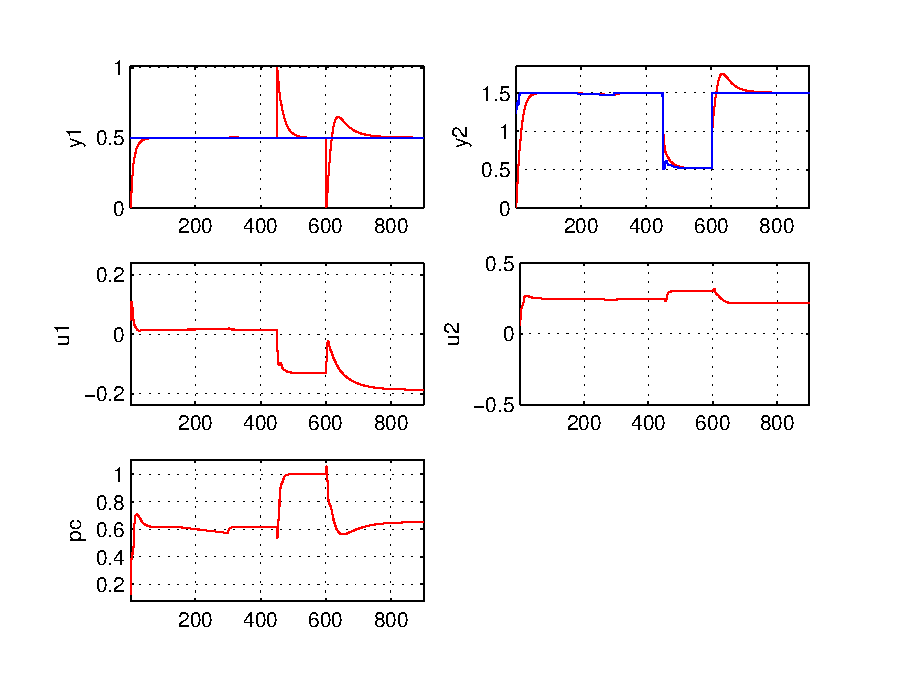
\includegraphics[width=7cm]{figuraeps}\\
  \caption{Tatulo de la figura 1. La figura es un fichero eps y gracias al paquete epstopdf se convierte automaticamente a pdf. Tambian se podraa convertir previamente la figura con un programa como Adobe Distiller}\label{fig1}
\end{figure}

\begin{figure}
\centering
  % Se pueden incluir figuras jpeg al compilar con PDFLatex
  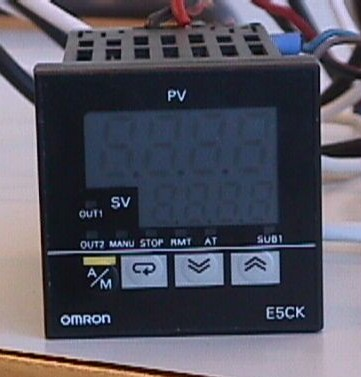
\includegraphics[width=3cm]{figurajpeg}\\
  \caption{Tatulo de la figura 2}\label{fig2}
\end{figure}


\section{Unidades}

Use el Sistema Internacional como unidades primarias. Se pueden usar
otras unidades como unidades secundarias (entre parantesis). Esto se
aplica a artaculos sobre almacenamiento de datos. Por ejemplo,
escriba ``$15 Gb/cm^2$'' ($100 Gb/in^2$). Se considera una excepcian
cuando las unidades inglesas se usan como identificadores
comerciales, como unidad de disco de 3.5 pulgadas. Evite mezclar
unidades del Sistema Internacional con el Sistema Cegesimal, tales
como corriente en amperios y campo magnatico en  oersteds. Esto a
menudo lleva a confusian porque las ecuaciones no son
dimensionalmente equiparables. Si debe usar unidades mezcladas,
especifique claramente las unidades para cada cantidad  en la
ecuacian. \citep{Abl:45} \citep{Abl:56} \citep{AbTaRu:54}

La unidad en el Sistema Internacional para la fuerza del campo
magnatico H es A/m. Sin embargo, si desea utilizar unidades de $T$,
o bien refiarase a densidad de flujo magnatico $B$ o fuerza del
campo magnatico simbolizado como $\mu_0 H$. Utilice el punto
centrado para separar unidades compuestas,  es decir, $A\cdot m^2$.

\section{Consejos atiles}

\subsection{Mas sobre Figuras y Tablas}

Las etiquetas de los ejes de las figuras son a menudo fuentes de
confusian. Utilice palabras en lugar de sambolos. Como ejemplo,
escriba la cantidad ``Magnetizacian,'' o ``Magnetizacian M,'' no
salo ``M.'' Ponga las unidades entre parantesis. No etiquete los
ejes anicamente con unidades. Como en la Fig. 1, por ejemplo,
escriba ``Magnetizacian (A/m)'' o ``Magnetizacian (A $\cdot$
m$^{-1}$),'' no salo ``A/m'' No etiquete los ejes con una relacian
de cantidades y unidades. Por ejemplo, escriba ``Temperatura (K),''
no ``Temperatura/K.''

Los multiplicadores pueden ser especialmente fuente de confusian.
Escriba``Magnetizacian (kA/m)'' o ``Magnetizacian ($10^3$ A/m).'' No
escriba ``Magnetizacian (A/m) $\times$ 1000'' porque el lector no
sabraa si la etiqueta del eje superior en la Fig. 1 es 16000 A/m o
0.016 A/m. Las etiquetas de las figuras deben ser legibles,
aproximadamente de 8 a 12 puntos.

\subsection{Referencias} % ATENCION: usar \citep en lugar de \cite para ajustarse al formato de RIAI.

La lista de referencias debe ser ordenada alfabaticamente
de acuerdo con el primer autor, con las siguientes laneas justificadas con la sangraa correspondiente.
Si existen diferentes publicaciones del mismo autor(es), astas deberan ser listadas en el orden del
aao de publicacian. Si hay mas de un artaculo del mismo autor en la misma fecha,
etiquatelas como a,b, etc. (Sanchez et al., 2000a, b). Por favor,
fajese que todas las referencias \citep{Garcia:2007}
listadas en este apartado \citep{Garcia:2008}
deben ser citadas directamente en el cuerpo del texto \citep{Garcia:2004}, \citep{Dog:58},
\citep{Keo:58},

\begin{figure}
\centering
  % Requires \usepackage{graphicx}
  % Se pueden incluir figuras pdf al compilar con PDFLatex
  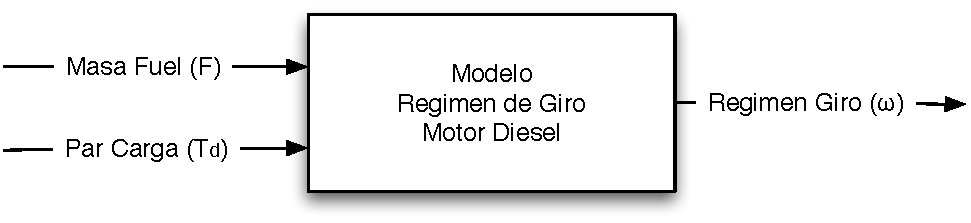
\includegraphics[width=7cm]{figurapdf}\\
  \caption{Tatulo de la figura 3}\label{fig3}
\end{figure}

Por favor, tenga en cuenta que las referencias al final de este
documento cumplen con el estilo anteriormente mencionado. Los
artaculos que no hayan sido publicados deben ser citados como ``no
publicado.'' Ponga en mayascula anicamente la primera palabra del
tatulo, excepto el caso de nombres propios y sambolos de elementos.

Si esta utilizando LaTeX, puede procesar una base de datos de bibliografaa externa o insertarla directamente en la seccian de referencias.
Las notas al pie de pagina se deben evitar en la medida de lo posible.

\subsection{Abreviaciones y Acranimos}

Defina las abreviaciones y acranimos la primera vez que se usan en
el texto, incluso despuas de ya hayan sido definidos en el resumen.
Abreviaciones tales como IFAC, SI, ac, y dc no necesitan ser
definidas. Abreviaciones que incorporen periodos no deben tener
espacios: escriba ``C.N.R.S.,'' no ``C. N. R. S.'' No utilice
abreviaciones en el tatulo salvo que sea inevitable (por ejemplo,
``RIAI'' en el tatulo de este artaculo).

\section{Mas sobre figuras}

Con el entorno \emph{figure*} se puede conseguir que una figura ocupe las dos columnas (ver figura \ref{mifigura}). Con el paquete \emph{subfigure} conseguimos una figura completa a partir de varios ficheros (como las subfiguras \ref{subfig1} y \ref{subfig2}).

\begin{figure*}[tb]
\centering
\subfigure[Tatulo Subfigura 11]{
   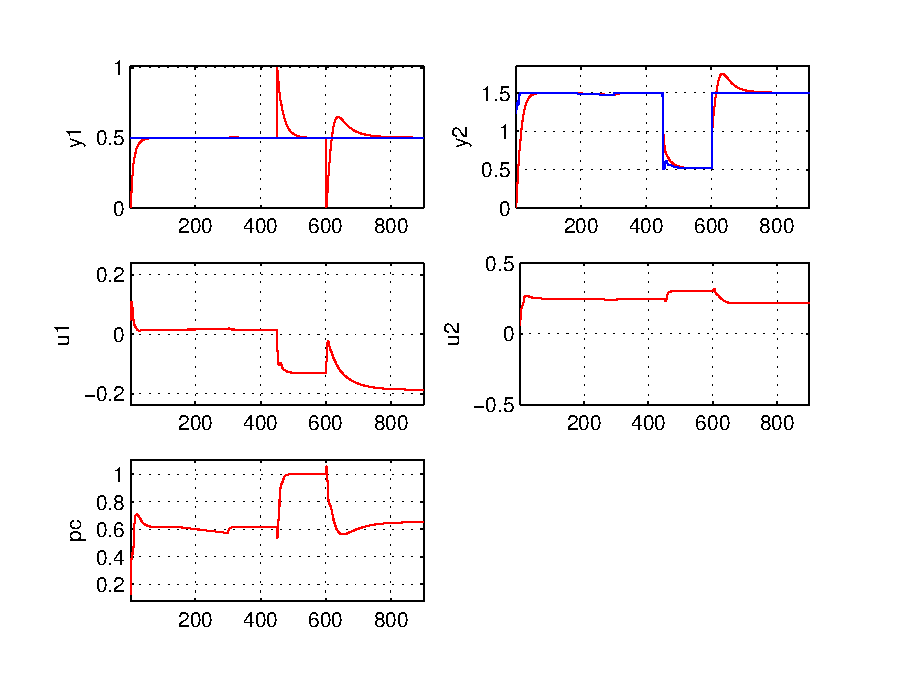
\includegraphics[scale =0.5] {figuraeps}
   \label{subfig1}
 }
 \subfigure[Tatulo Subfigura 2]{
   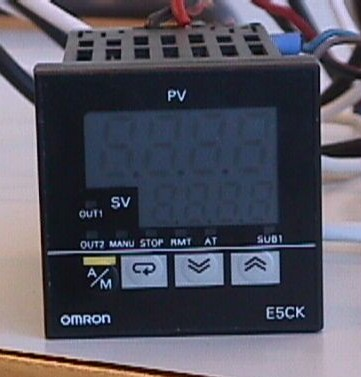
\includegraphics[scale =0.35] {figurajpeg}
   \label{subfig2}
 }

\label{mifigura}
\caption{Tatulo global para la figura.}
\end{figure*}

\subsection{Ecuaciones}

Numere las ecuaciones consecutivamente con nameros de ecuaciones
entre parantesis justificado al margen derecho, como en \eqref{e2}.
Primero use el editor de ecuaciones para crear la ecuacian. Despuas
seleccione el estilo ``Equation''. Presione la tecla de tabulador y
escriba el namero de ecuacian entre parantesis. Para hacer sus
ecuaciones mas compactas, puede usar el solidus ( / ), la funcian
exp, o los exponentes apropiados. Utilice parantesis para evitar
ambigaedades en los denominadores. Ponga signos de puntuacian en las
ecuaciones cuando formen parte de una frase, como en

\begin{equation} \label{e2}
\begin{array}{ll}
\int_0^{r_2} & F (r, \varphi ) dr d\varphi = [\sigma r_2 / (2 \mu_0 )] \\
& \cdot \int_0^{\inf} exp(-\lambda |z_j - z_i |) \lambda^{-1} J_1 (\lambda  r_2 ) J_0 (\lambda r_i ) d\lambda
\end{array}
\end{equation}

Asegarese de que los sambolos de su ecuacian han sido definidos
antes de que la ecuacian aparezca o inmediatamente despuas. Ponga en
cursiva los sambolos (T podraa referirse a la temperatura, pero T es
la unidad tesla). Refiarase a ``(1),'' no ``Ec. (1)'' o ``ecuacian
(1),'' excepto al principio de la frase: ``La ecuacian (1) es ...
.''

\subsection{Otras Recomendaciones}

Utilice un espacio tras los periodos y dos puntos. Evite utilizar
participios, tales como, ``Utilizando (1), se calcula el
potencial.'' [No esta claro quien o qua usa (1).] En su lugar
escriba ``El Potencial fue calculado empleando (1),'' o ``Empleando
(1), se calcula el potencial.''

\section{Conclusian}

Una seccian de conclusiones no es necesaria. Sin embargo, las conclusiones pueden revisar los puntos mas importantes de un artaculo, pero no debe replicarse el resumen en las conclusiones. Las conclusiones pueden tratar sobre la importancia del trabajo realizado o sugerir aplicaciones o trabajos futuros.

Repetido. Una seccian de conclusiones no es necesaria. Sin embargo, las conclusiones pueden revisar los puntos mas importantes de un artaculo, pero no debe replicarse el resumen en las conclusiones. Las conclusiones pueden tratar sobre la importancia del trabajo realizado o sugerir aplicaciones o trabajos futuros.

Repetido. Una seccian de conclusiones no es necesaria. Sin embargo, las conclusiones pueden revisar los puntos mas importantes de un artaculo, pero no debe replicarse el resumen en las conclusiones. Las conclusiones pueden tratar sobre la importancia del trabajo realizado o sugerir aplicaciones o trabajos futuros.
%%%%%%%%%%%%%%%%%%%%%%%%%%%%%%%%%%%%%%%%%%%%%%%%%%%%%%%%%%%%%%%%%%%%%%%%%%%%%%%%%%%%%%%%
%% ATENCION AUTORES: ESTA SECCION ES OBLIGATORIA
%%%%%%%%%%%%%%%%%%%%%%%%%%%%%%%%%%%%%%%%%%%%%%%%%%%%%%%%%%%%%%%%%%%%%%%%%%%%%%%%%%%%%%%%

\section*{English Summary}

\textbf{Paper title in English, bold style.}\\

\noindent \textbf{Abstract}\\

Many young learners are required to write essays in English. While most of these students also write essays for other courses in their native language, they often feel hesitant when writing essays in English. This series of four lessons is designed to help students become familiar with writing an essay in English. The first lesson is designed to give students an overview of basic essay writing style. The final three lessons focus on developing skills that are used when analyzing texts as the basis of their essays.\\

\noindent \emph{Keywords:}\\

Keyword 1, keyword 2, keyword 3.
%%%%%%%%%%%%%%%%%%%%%%%%%%%%%%%%%%%%%%%%%%%%%%%%%%%%%%%%%%%%%%%%%%%%%%%%%%%%%%%%%%%%%%%%%%
\section*{Agradecimientos}

Este trabajo ha sido realizado parcialmente gracias al apoyo de la Agencia Nacional (los agradecimientos de financiacian y apoyos han de ser incluidos aqua).

\label{}

%% The Appendices part is started with the command \appendix;
%% appendix sections are then done as normal sections
%% \appendix

%% \section{}
%% \label{}

%% References
%%
%% Following citation commands can be used in the body text:
%% Usage of \cite is as follows:
%%   \cite{key}         ==>>  [#]
%%   \cite[chap. 2]{key} ==>> [#, chap. 2]
%%


%% References with BibTeX database:

\bibliographystyle{elsarticle-harv}
%%\bibliography{riaibib}

%% Authors are advised to use a BibTeX database file for their reference list.
%% The provided style file elsarticle-num.bst formats references in the required Procedia style

%% For references without a BibTeX database:

%%\begin{thebibliography}{01}

%% \bibitem must have the following form:
%%   \bibitem{key}...
%%

% \bibitem{}

%%\bibitem[{Able(1945)}]{Abl:45}
%%Able, B., 1945. Nombre del artículo. Nombre de la revista 35, 123--126.

\begin{thebibliography}{7}
\expandafter\ifx\csname natexlab\endcsname\relax\def\natexlab#1{#1}\fi
\expandafter\ifx\csname url\endcsname\relax
  \def\url#1{\texttt{#1}}\fi
\expandafter\ifx\csname doi\endcsname\relax
  \def\doi#1{\texttt{#1}}\fi
\expandafter\ifx\csname urlprefix\endcsname\relax\def\urlprefix{URL: }\fi
\expandafter\ifx\csname doiprefix\endcsname\relax\def\doiprefix{DOI: }\fi

\bibitem[{Able(1945)}]{Abl:45}
Able, B., 1945. Nombre del artículo. Nombre de la revista 35, 123--126.
\newline\doiprefix\doi{10.3923/ijbc.2010.190.202}

\bibitem[{Able(1956)}]{Abl:56}
Able, B., 1956. Nombre del artículo. Nombre de la revista 135, 7--9.
\newline\doiprefix\doi{10.3923/ijbc.2010.190.202}

\bibitem[{Baker(1963{\natexlab{b}})}]{Bak:63b}
Baker, R., 1963{\natexlab{b}}. Nombre del artículo. Nombre de la revista 34,
  184--186.
\newline\doiprefix\doi{10.3923/ijbc.2010.190.202}

\bibitem[{Charlie y Routh(1966)}]{ChaRou:66}
Charlie, F., Routh, M., 1966. Nombre del artículo. Nombre de la revista 66,
  267--269.
\newline\doiprefix\doi{10.3923/ijbc.2010.190.202}

\bibitem[{García y Martínez(2008)}]{Garcia:2008}
García, F., Martínez, R., 2008. Nombre del artículo. Nombre de la revista
  número, {}números de página.
\newline\doiprefix\doi{10.3923/ijbc.2010.190.202}

\bibitem[{Soukhanov(1992)}]{Heritage:92}
Soukhanov, A.~H. (Ed.), 1992. Nombre de la editorial.


 \end{thebibliography}

\appendix
\section{Primer Apandice}    % Capa Apandice debe tener un tatulo corto.
Este texto esta repetido. Si utiliza Word, use o bien Microsoft Editor de Ecuaciones o
MathType  para las ecuaciones de su artaculo (Insertar | Objeto |
Crear Nuevo | Microsoft Editor de Ecuaciones o Ecuacian MathType).
No debe seleccionar la opcian ``Flotar'' sobre el texto. Por
supuesto, LaTeX gestiona las ecuaciones a travas de macros
pre-programadas.

\section{Segundo Apandice}

Este texto esta repetido. Use el Sistema Internacional como unidades primarias. Se pueden usar
otras unidades como unidades secundarias (entre parantesis). Esto se
aplica a artaculos sobre almacenamiento de datos. Por ejemplo,
escriba ``$15 Gb/cm^2$'' ($100 Gb/in^2$). Se considera una excepcian
cuando las unidades inglesas se usan como identificadores
comerciales, como unidad de disco de 3.5 pulgadas. Evite mezclar
unidades del Sistema Internacional con el Sistema Cegesimal, tales
como corriente en amperios y campo magnatico en  oersteds. Esto a
menudo lleva a confusian porque las ecuaciones no son
dimensionalmente equiparables. Si debe usar unidades mezcladas,
especifique claramente las unidades para cada cantidad  en la
ecuacian.

La unidad en el Sistema Internacional para la fuerza del campo
magnatico H es A/m. Sin embargo, si desea utilizar unidades de $T$,
o bien refiarase a densidad de flujo magnatico $B$ o fuerza del
campo magnatico simbolizado como $\mu_0 H$. Utilice el punto
centrado para separar unidades compuestas,  es decir, $A\cdot m^2$.

\section{Tercer Apandice}

\subsection{Mas sobre Figuras y Tablas}

Este texto esta repetido. Las etiquetas de los ejes de las figuras son a menudo fuentes de
confusian. Utilice palabras en lugar de sambolos. Como ejemplo,
escriba la cantidad ``Magnetizacian,'' o ``Magnetizacian M,'' no
salo ``M.'' Ponga las unidades entre parantesis. No etiquete los
ejes anicamente con unidades. Como en la Fig. 1, por ejemplo,
escriba ``Magnetizacian (A/m)'' o ``Magnetizacian (A $\cdot$
m$^{-1}$),'' no salo ``A/m'' No etiquete los ejes con una relacian
de cantidades y unidades. Por ejemplo, escriba ``Temperatura (K),''
no ``Temperatura/K.''

Los multiplicadores pueden ser especialmente fuente de confusian.
Escriba``Magnetizacian (kA/m)'' o ``Magnetizacian ($10^3$ A/m).'' No
escriba ``Magnetizacian (A/m) $\times$ 1000'' porque el lector no
sabraa si la etiqueta del eje superior en la Fig. 1 es 16000 A/m o
0.016 A/m. Las etiquetas de las figuras deben ser legibles,
aproximadamente de 8 a 12 puntos.

\end{document}

%%
%% End of file `ejemplo latex RIAI.tex'.